\newpage
\section{Przechowywanie danych}

Poszczególne mikroserwisy odwołują się do różnych źródeł danych w celu uzyskania 
wymaganych informacji. W tej pracy wykorzystano dwa różne sposoby przechowywania 
informacji:

\begin{itemize} % lista nienumerowana
    \item Relacyjna baza danych MySQL
    \item Baza danych szeregów czasowych InfluxDB
\end{itemize}

Sekcja 5.1 przybliża szczegóły dotyczące utworzonych modeli danych oraz sposobu 
przechowywania informacji w relacyjnej bazie danych. Podrozdziały 5.1.1 - 5.1.5 przedstawiają
szczegółowo kolejne schematy danych. Sekcja 5.2 jest poświęcona przechowywaniu
wykonanych przez czujniki pomiarów w bazie danych szeregów czasowych.

\subsection{MySQL}

Relacyjna baza danych MySQL oferuje szybki, wielowątkowy serwer bazodanowy w oparciu 
o język SQL (ang. \textit{Structured Query Language})
\cite{mysql2022}. Została ona wybrana ze względu na to, że 
jest produktem typu open-source dostępnym na licencji GNU (ang. \textit{general public license}). 

Dobrą praktyką, którą warto mieć na uwadze podczas tworzenia systemu opartego na 
architekturze mikrousługowej, jest zapewnienie dostępu do konkretnego modelu danych tylko 
jednemu mikroserwisowi, który następnie może udostępniać posiadane informacje przy pomocy odpowiednio 
skonfigurowanego API (ang. \textit{Application Programming Interface}) \cite{richardson2021}. Takie podejście umożliwia zachowanie luźnego 
sprzężenia między mikroserwisami. W konsekwencji należy utworzyć oddzielne modele 
danych, zwane schematami, które mogą być zarządzane przez pojedynczy mikroserwis.

W ramach utworzonego serwera bazodanowego zostały wdrożone następujące schematy:

    \begin{xltabular}{1\textwidth} { 
        | >{\raggedright\arraybackslash}c        
        | >{\raggedright\arraybackslash}X | }
        \caption{Utworzone schematy bazodanowe} \label{tab:schematy-bazodanowe} \\
        \hline
       Nazwa schematu & Funkcja \\
       \hline
       Addresses (adresy) & 
       Przechowuje dane dotyczące adresów \\
       \hline
       Facilities (organizacje) &
       Przechowuje dane dotyczące organizacji oraz budynków \\
       \hline
       Identity (użytkownicy) &
       Przechowuje dane użytkowników \\
       \hline
       Policies (reguły) &
       Przechowuje dane dotyczące reguł określających oczekiwaną wartość mierzonych 
       parametrów \\
       \hline
       Sensors (sensory) & 
       Przechowuje dane dotyczące wykorzystywanych sensorów \\
       \hline
    \end{xltabular}

\subsubsection{Schemat adresów}

Rysunek \ref{fig:diagram-adresy} przedstawia diagram UML modelu danych adresów. 

\begin{figure}[H]
    \centering
    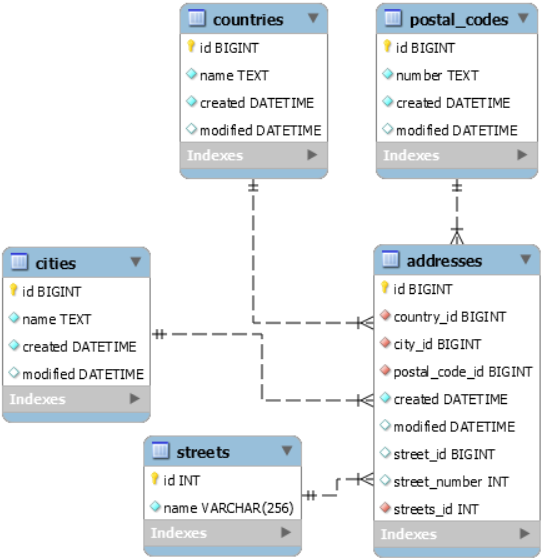
\includegraphics[width=0.8\textwidth]{addresses_diagram.png}
    \caption{Diagram modelu danych adresów. Opracowanie własne}
    \label{fig:diagram-adresy}
\end{figure}

Schemat adresów składa się z encji opisanych w tabeli \ref{tab:encje-adresow}:

    \begin{xltabular}{1\textwidth} { 
        | >{\raggedright\arraybackslash}c        
        | >{\raggedright\arraybackslash}X | }
        \caption{Encje w schemacie adresów} \label{tab:encje-adresow} \\
        \hline
       Nazwa encji & Przechowywane dane \\
       \hline
       Addresses & 
       Encja główna, zawiera odwołania do kraju, miasta, kodu pocztowego, numeru ulicy 
       oraz numeru budynku \\
       \hline
       Cities & Miasto \\
       \hline
       Countries & Kraj \\
       \hline
       Postal codes & Kod pocztowy \\
       \hline
       Streets & Ulica \\
       \hline
    \end{xltabular}

Związki między poszczególnymi encjami zostały opisane w tabeli \ref{tab:zwiazki-adresy}.


\begin{xltabular}{1\textwidth} { 
        | >{\arraybackslash}c    
        | >{\arraybackslash}c
        | >{\arraybackslash}c     
        | >{\arraybackslash}X | }
        \caption{Związki między encjami w schemacie adresów} \label{tab:zwiazki-adresy} \\
        \hline
    \multicolumn{2}{|c|}{Relacja} & Typ związku & Opis \\
    \hline
    Addresses & Countries & 1:N & 
    Każdy kraj może występować w wielu adresach \\
    \hline
    Addresses & Cities & 1:N & 
    Każde miasto może występować w wielu adresach \\
    \hline
    Addresses & Postal codes & 1:N 
    & Każdy kod pocztowy może występować w wielu adresach \\
    \hline
    Addresses & Strees & 1:N & 
    Każda ulica może występować w wielu adresach \\
    \hline
    \end{xltabular}

\begin{figure}[H]
    \centering
    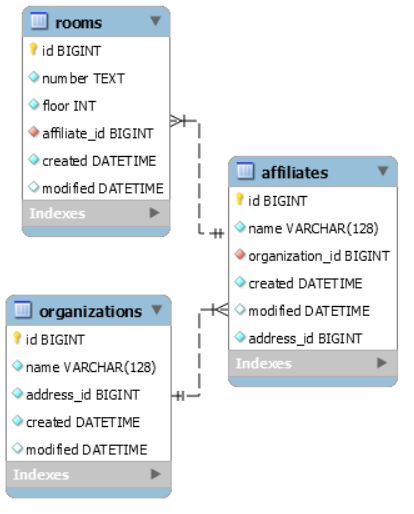
\includegraphics[width=0.7\textwidth]{facilities_diagram.png}
    \caption{Diagram modelu danych organizacji. Opracowanie własne}
    \label{fig:diagram-organizacje}
\end{figure}

\subsubsection{Schemat organizacji}

Rysunek \ref{fig:diagram-organizacje} przedstawia diagram UML modelu danych organizacji. 

Schemat organizacji składa się z encji opisanych w tabeli \ref{tab:encje-organizacji}:

    \begin{xltabular}{1\textwidth} { 
        | >{\raggedright\arraybackslash}c        
        | >{\raggedright\arraybackslash}X | }
        \caption{Encje w schemacie organizacji} \label{tab:encje-organizacji} \\
        \hline
       Nazwa encji & Przechowywane dane \\
       \hline
       Affiliates & 
       Oddziały danej organizacji \\
       \hline
       Rooms & Pomieszczenia w oddziałach \\
       \hline
       Organizations & Organizacje \\
       \hline
    \end{xltabular}

Związki między poszczególnymi encjami zostały opisane w tabeli \ref{tab:zwiazki-organizacje}.

\begin{xltabular}{1\textwidth} { 
        | >{\arraybackslash}c   
        | >{\arraybackslash}c
        | >{\arraybackslash}c     
        | >{\arraybackslash}X | }
        \caption{Związki między encjami w schemacie organizacji} \label{tab:zwiazki-organizacje} \\
        \hline
    \multicolumn{2}{|c|}{Relacja} & Typ związku & Opis \\
    \hline
    Organizations & Affiliates & 1:N & 
    Każdy organizacja może posiadać wiele oddziałów \\
    \hline
    Affiliates & Rooms & 1:N & 
    Każdy oddział może posiadać wiele pomieszczeń \\
    \hline
    \end{xltabular}

\subsubsection{Schemat reguł}

Rysunek \ref{fig:diagram-reguly} przedstawia diagram UML modelu danych reguł. 

Schemat reguł składa się z encji opisanych w tabeli \ref{tab:encje-regul}:

    \begin{xltabular}{1\textwidth} { 
        | >{\raggedright\arraybackslash}c        
        | >{\raggedright\arraybackslash}X | }
        \caption{Encje w schemacie reguł} \label{tab:encje-regul}\\
        \hline
       Nazwa encji & Przechowywane dane \\
       \hline
       Room policies & 
       Encja główna, zawiera odwołania do kategorii oraz oczekiwanych warunków. Przechowuje 
       okres obowiązywania danej reguły \\
       \hline
       Room policy categories & Kategorie reguł \\
       \hline
       Expected room conditions & Oczekiwane warunki w pomieszczeniu \\
       \hline
    \end{xltabular}

\begin{figure}[H]
    \centering
    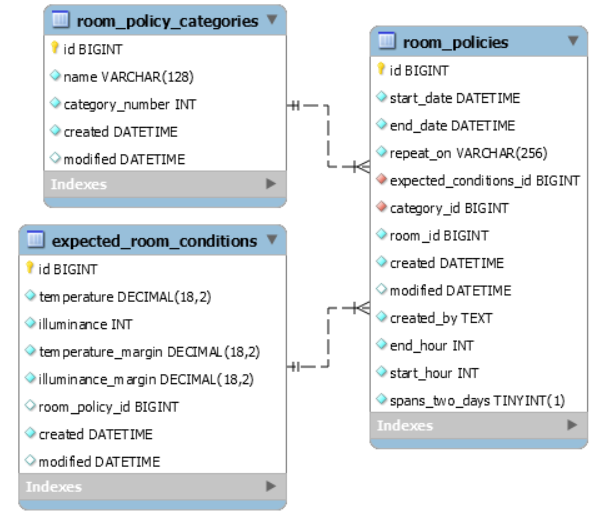
\includegraphics[width=0.8\textwidth]{policies_diagram.png}
    \caption{Diagram modelu danych reguł. Opracowanie własne}
    \label{fig:diagram-reguly}
\end{figure}

Związki między poszczególnymi encjami zostały opisane w tabeli \ref{tab:zwiazki-reguly}.

\begin{xltabular}{1\textwidth} { 
        | >{\arraybackslash}c    
        | >{\arraybackslash}c
        | >{\arraybackslash}c     
        | >{\arraybackslash}X | }
        \caption{Związki między encjami w schemacie reguł} \label{tab:zwiazki-reguly} \\
        \hline
    \multicolumn{2}{|c|}{Relacja} & Typ związku & Opis \\
    \hline
    Room policies & Room policy categories & 1:N & 
    Każda kategoria może być przypisana wielu regułom \\
    \hline
    Room policies & Expected room conditions & 1:N & 
    Ten sam zbiór oczekiwanych warunków może być przypisany do wielu reguł \\
    \hline
    \end{xltabular}

\subsubsection{Schemat sensorów}

Rysunek \ref{fig:diagram-sensory} przedstawia diagram UML modelu danych sensorów. 

\begin{figure}[H]
    \centering
    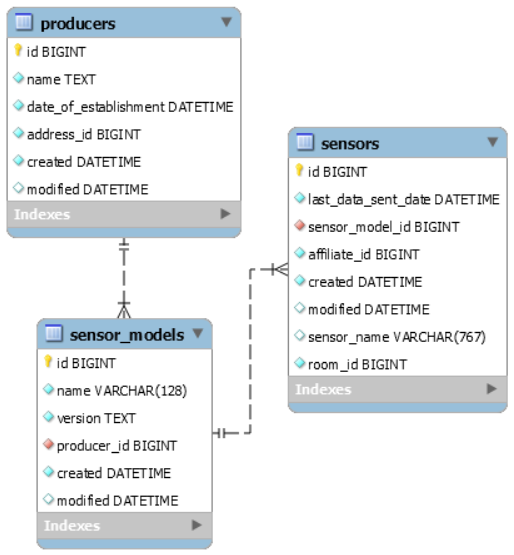
\includegraphics[width=0.8\textwidth]{sensors_diagram.png}
    \caption{Diagram modelu danych sensorów. Opracowanie własne}
    \label{fig:diagram-sensory}
\end{figure}

Schemat sensorów składa się z encji opisanych w tabeli \ref{tab:encje-sensorow}:

    \begin{xltabular}{1\textwidth} { 
        | >{\raggedright\arraybackslash}c        
        | >{\raggedright\arraybackslash}X | }
        \caption{Encje w schemacie sensorów} \label{tab:encje-sensorow} \\
        \hline
       Nazwa encji & Przechowywane dane \\
       \hline
       Sensors & Szczegóły dotyczące danego sensora \\
       \hline
       Sensor models & Model sensora \\
       \hline
       Producers & Producent sensorów \\
       \hline
    \end{xltabular}

Związki między poszczególnymi encjami zostały opisane w tabeli \ref{tab:zwiazki-sensory}.

\begin{xltabular}{1\textwidth} { 
        | >{\arraybackslash}c    
        | >{\arraybackslash}c
        | >{\arraybackslash}c     
        | >{\arraybackslash}X | }
        \caption{Związki między encjami w schemacie sensorów} \label{tab:zwiazki-sensory} \\
        \hline
    \multicolumn{2}{|c|}{Relacja} & Typ związku & Opis \\
    \hline
    Sensor models & Producers & 1:N & 
    Każdy producent może oferować wiele modeli sensorów \\
    \hline
    Sensor models & Sensors & 1:N & 
    Każdy model może być wypordukowany wielokrotnie \\
    \hline
    \end{xltabular}

\subsubsection{Schemat użytkowników}

Rysunek \ref{fig:diagram-uzytkownicy} przedstawia diagram UML modelu danych użytkowników. 

\begin{figure}[H]
    \centering
    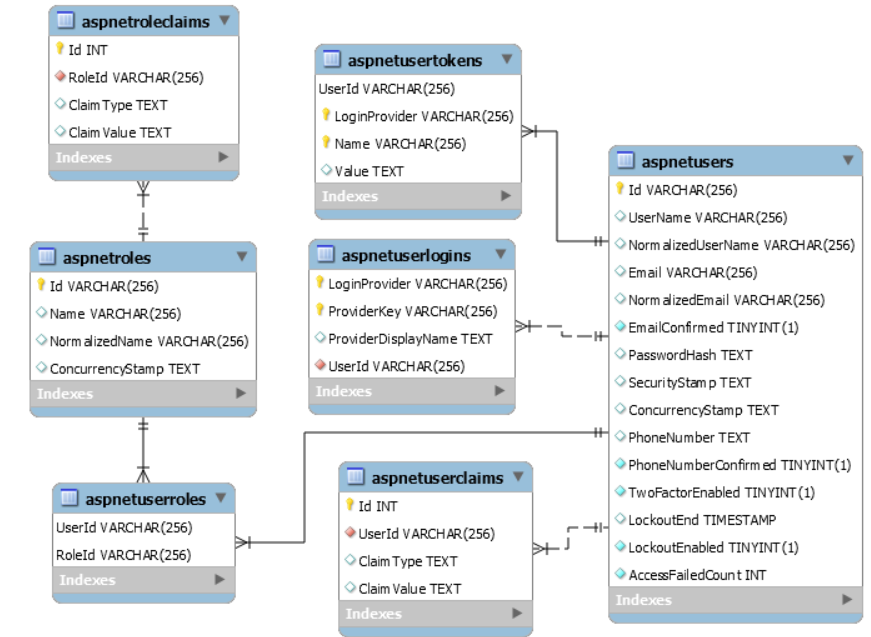
\includegraphics[width=1\textwidth]{users_diagram.png}
    \caption{Diagram modelu danych użytkowników. Opracowanie własne}
    \label{fig:diagram-uzytkownicy}
\end{figure}

Schemat użytkowników został oparty na schemacie oferowanym przez Microsoft 
\parencite{vickers2021} i składa się z następujących encji:

    \begin{xltabular}{1\textwidth} { 
        | >{\raggedright\arraybackslash}c        
        | >{\raggedright\arraybackslash}X | }
        \caption{Encje w schemacie użytkowników} \label{tab:encje-uzytkownicy}\\
        \hline
       Nazwa encji & Przechowywane dane \\
       \hline
       Asnetusers & Reprezentuje użytkownika \\
       \hline
       Aspnetroles & Reprezentuje rolę użytkownika w systemie \\
       \hline
       Aspnetuserlogins & Łączy użytkownika z loginem \\
       \hline
       Aspnetusertokens & Reprezentuje token uwierzytelniający dla użytkownika \\
       \hline
       Aspnetuserclaims & Reprezentuje prawa, które posiada użytkownik \\
       \hline
       Aspnetroleclaims & Reprezentuje prawa gwarantowane dla wszystkich użytkowników
       pełniących daną rolę \\
       \hline
       Aspnetuserroles & Łączy użytkowników z poszczególnymi rolami \\
       \hline
    \end{xltabular}

Związki między poszczególnymi encjami zostały opisane w tabeli \ref{tab:zwiazki-uzytkownicy}.

\begin{xltabular}{1\textwidth} { 
        | >{\arraybackslash}c    
        | >{\arraybackslash}c
        | >{\arraybackslash}c     
        | >{\arraybackslash}X | }
        \caption{Związki między encjami w schemacie użytkowników} \label{tab:zwiazki-uzytkownicy} \\
        \hline
    \multicolumn{2}{|c|}{Relacja} & Typ związku & Opis \\
    \hline
    Aspnetusers & Aspnetuserlogins & 1:N & 
    Każdemu użytkownikowi może być przypisanych wiele loginów \\
    \hline
    Aspnetusers & Aspnetusertokens & 1:N & 
    Każdemu użytkownikowi może być przypisanych wiele tokenów \\
    \hline
    Aspnetusers & Aspnetuserroles & 1:N &
    Każdy użytkownik może pełnić wiele ról \\
    \hline
    Aspnetusers & Aspnetuserclaims & 1:N &
    Każdy użytkownik może posiadać wiele praw \\
    \hline
    Aspnetroles & Aspnetroleclaims & 1:N &
    Każdej roli może być przypisanych wiele praw \\
    \hline
    Aspnetroles & Aspnetuserroles & 1:N &
    Każda rola może być pełniona przez wielu użytkowników \\
    \hline
    \end{xltabular}

\subsection{InfluxDB}

InfluxDB jest bazą danych szeregów czasowych służącą do przechowywania metryk 
i szeregów czasowych \cite{influxdb2022}. Umożliwia efektywne przechowywanie 
miliardów rekordów danych 
dzięki stosowaniu kompresji danych, oferuje także język zapytań pozwalający 
przeprowadzać kompleksowe analizy uzyskanych informacji. Dodatkową funkcjonalnością 
wyróżniającą tą bazę od standardowych relacyjnych baz danych jest możliwość 
zdefiniowania czasu, po którym rekordy będą usuwane. Można w ten sposób określić na 
przykład, że baza powinna przechowywać tylko rekordy z ostatniego miesiąca.

W tej pracy inżynierskiej baza danych szeregów czasowych została wykorzystana do 
przechowywania danych zbieranych z czujników temperatury oraz natężenia światła. 
Przychodzące informacje są zapisywane w kolejnych rekordach, które zawierają 
następujące parametry:

    \begin{xltabular}{1\textwidth} { 
        | >{\raggedright\arraybackslash}c 
        | >{\raggedright\arraybackslash}X | }
        \caption{Parametry pojedynczego rekordu przechowującego pomiar} \label{tab:parametry-pomiaru}\\
        \hline
       Parametr & Znaczenie \\
       \hline
       time & Czas otrzymania danych \\
       \hline
       field & Rodzaj danych \\
       \hline
       value & Zmierzona wartość \\
       \hline
    \end{xltabular}

    Domyślnie czas jest zapisywany z dokładnością do nanosekund. W tej pracy zostały
    zdefiniowane dwa rodzaje danych: \textit{temperature} dotyczące informacji o temperaturze 
    oraz \textit{illuminance} dotyczące informacji o natężeniu światła.